
%----------------------------------------------------------------
%
%  File    :  aufbau_lte.tex
%
%  Authors :  Eisenhut
% 
%  Created :  7 Sept 2019
% 
%  Changed :  11 Sept 2019
% 
%---------------------------------------------------------------


\section{Aufbau LTE}
\label{sec:aufbau}
\subsection{LTE Entwicklung}
\label{subsec:LTE Entwicklung}
LTE ist im Release (R)\abk{R}{Release}8 im Dezember 2008 von der Third Generation Partnership Project (3GPP) \abk{3GPP}{Third Generation Partnership Project} eingefroren worden und stellt die Basis des ersten LTE Equipments dar. Der R8 stellt eine Verbesserung des 3G Standards dar, zählt aber zu 3G \cite[S. 32ff]{Zoi09}. Erst LTE R10, auch LTE+ oder LTE Advanced genannt, als Standard von der 3GPP oder der International Mobile Telecommunications (IMT)\abk{IMT}{International Mobile Telecommunications}-Advanced Standard der International Telecommunication Union Radiocommunication Sector (ITU-R)\abk{ITU-R}{International Telecommunication Union Radiocommunication Sector} erfüllen die Anforderungen von 4G und werden in dieser Arbeit vereinfachend LTE genannt \cite{Wan13}.

Der Treiber bei der Entwicklung von LTE war die Erhöhung der Kapazität. Es werden kosteneffizient höhere Bitraten (Download~(DL)\abk{DL}{Download}: 3\,Gbit/s, Upload (UL)\abk{UL}{Upload}: 1,5\,Gbit/s\abk{Gbit/s}{Gigabit pro Sekunde}) ermöglicht. Dies wird durch höhere Link Spektrale Effizienz bei R10 von 30\,(bit/s)/Hz im Gegensatz von R8 mit 16\,(bit/s)/Hz\abk{Hz}{Hertz} erreicht. Dadurch erhöht sich die Anzahl der möglichen, gleichzeitig aktiven Teilnehmer des Netzes. Ebenso erhöht sich die System Spektrale Effizienz bei R10 für den DL mit Multiple Input–Multiple Output (MIMO) auf 2,4\,(bit/s)/Hz/Zelle. Im Gegensatz zu 3G/LTE wird dies durch Carrier Aggregation (CA)\abk{CA}{Carrier Aggregation}, dem gestiegenen Einsatz von Multi-Antennen Techniken und Relay Nodes (RN)\abk{RN}{Relay Nodes} erreicht \cite{Wan13}. Zurzeit ist R15 der höchste stabile Release der 3GPP für LTE. Ab R12 werden die Releases als LTE Advanced Pro und 4,5G genannt, um die  Annäherung an den neuen 5G Standard zu symbolisieren. LTE ist ein Markenname des European Telecommunications Standards Institute (ETSI)\abk{ETSI}{European Telecommunications Standards Institute}. R15 bietet eine höchste Link Spektrale Effizienz von 30\,(bit/s)/Hz beim DL und 15\,(bit/s)/Hz bei einer DL Antennenkonfiguration von 8x8 und UL 4x4. Bei 4x4 wird für den DL eine System Spektrale Effizienz von 0,12\,(bit/s)/Hz/Zelle/Teilnehmer, wenn sich 10 Teilnehmer in der Zelle befinden, erreicht. Das Voice over Internet Protocol (VoIP)\abk{VoIP}{Voice over Internet Protocol} ist in jeder Antennenkonfiguration möglich. Abhängig vom Frequenzband sind Spitzengeschwindigkeiten der mobilen Endgeräte (zB Handy, Datenwürfel) technisch User Equipment (UE)\abk{UE}{User Equipment} genannt von 350 bis 500\,km/h\abk{km/h}{Kilometer pro Stunde} möglich \cite{GPP18}.
\subsection{Architektur LTE}
\label{subsec:architektur}
Die Daten werden paketorientiert mit dem Internet Protocol~(IP)\abk{IP}{Internet Protocol} übermittelt. Die Architektur besteht aus vier Blöcken. Das UE ist per Funk mit dem Evolved Universal Terrestrial Radio Access (E-UTRA)\abk{E-UTRAN}{Evolved Universal Terrestrial Radio Access Network} verbunden. Das E-UTRA ist über den Evolved NodeB (eNodeB)\abk{eNodeB}{Evolved NodeB} mittels Leitungen mit dem Evolved Packet Core (EPC)\abk{EPC}{Evolved Packet Core} verbunden.
\begin{figure}[H]
	\centering
	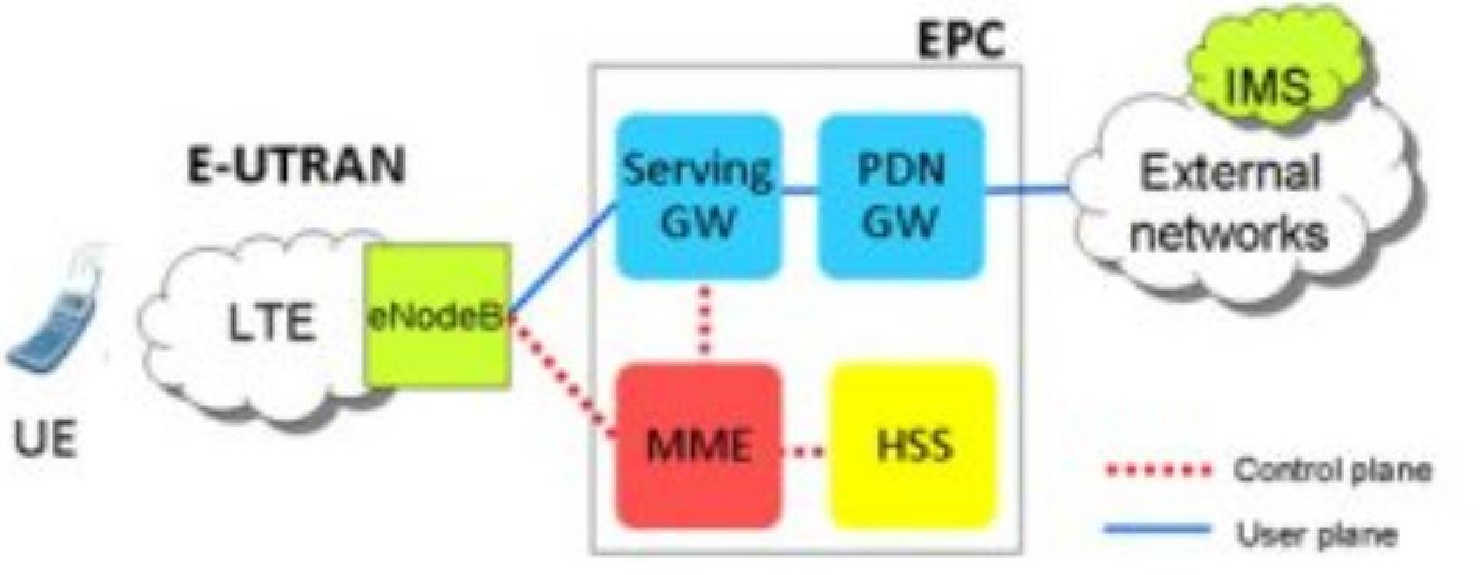
\includegraphics[width=1\linewidth]{LTE_Architektur}
	\caption{Architektur LTE \protect\cite{Fir19}}
	\label{fig:bildarchitektur}
\end{figure}
Die Signalisierungsdaten und die Mediendaten werden separat übermittelt. Die Mediendaten werden der User Plane und die Signalisierungsdaten der Control Plane übergeben. Leitungen verbinden das EPC mit externen Telefonnetzen sowie Datennetzen, dem IP Multimedia Core Network Subsystem (IMS\abk{IMS}{IP Multimedia Core Network Subsystem} , siehe Abb\abk{Abb}{Abbildung} \ref{fig:bildarchitektur}) \cite{Fir19}.
E-UTRAN wird auch Radio Access Network (RAN)\abk{RAN}{Radio Access Network} und das EPC Core Network (CN)\abk{CN}{Core Network} genannt. System Architecture Evolution (SAE) ist der Standard der Architektur von der 3GPP für das CN. LTE und SAE beinhalten das Evolved Packet System (EPS)\abk{EPS}{Evolved Packet System}. Dies bietet eine nahtlose Benutzung des IP vom UE zum Packet Data Network (PDN)\abk{PDN}{Packet Data Network} und gestattet sowohl Quality of Service (QoS)\abk{QoS}{Quality of Service} als auch IP Dienste wie zB VoIP. Es können mehrere Kanäle mit unterschiedlichem QoS von verschiedenen PDN's für unterschiedliche Dienste angeboten werden \cite{Ses11}.
\subsection{Logische Komponenten}
\label{subsec:logkomponenten}
\subsubsection{User Equipment}
\label{subsubsec:ue}
Ab R12 sind der DL und UL in eigenen Kategorien getrennt spezifiziert. Die DL und UL Kategorien können unterschiedlich sein \cite{GPP19}. Das UE ist nicht Teil der zu beschaffenden Infrastruktur. 
\subsubsection{E-UTRAN}
\label{subsubsec:eutran}
Die Architektur im E-UTRAN (siehe Abb. \ref{fig:eutranarchitektur}) ist bewusst flach gehalten und besteht nur aus miteinander über das X2 Protokoll kommunizierenden eNodeB's. Auch die Übergabe von UE an andere eNodeB's regeln diese ressourcenschonend alleine, ohne einen zentralen Controller. Über das S1 Protokoll kommuniziert ein eNodeB mit den CN Knoten. Der Mobility Management Entity (MME)\abk{MME}{Mobility Management Entity} werden die Signalisierungsdaten und dem Serving Gateway (SGW)\abk{SGW}{Serving Gateway} die Mediendaten übergeben. Mit dem S1-flex Protololl versorgen mehrere CN Knoten (MME/S-GWs) eine gemeinsame Region (Pool Area) durch Vernetzung mit den eNodeB's, dem MME/S-GW Pool. Die UE's einer Zelle, die von einem eNodeB betreut werden, sind von mehreren CN-Knoten unterstützt. Das verhindert einen Single Point of Failure bei den CN-Knoten und erlaubt Load Balancing. Der UE Kontext verbleibt normalerweise bei einem MME, solange sich die UE in der selben Pool Area befindet \cite{Ses11}.
\begin{figure}[H]
	\centering
	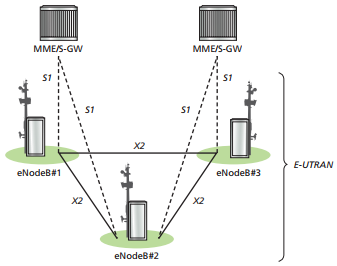
\includegraphics[width=1\linewidth]{images/E_UTRAN_Architektur}
	\caption[]{E-Utran Architektur \protect\cite{Ses11}}
	\label{fig:eutranarchitektur}
\end{figure}
Die Schnittstelle zum UE sind die Access Stratum (AS)\abk{AS}{Access Stratum} Protokolle \cite[S. 131]{Sau06}. Das E-UTRAN ist für das Radio Resource Management (RRM)\abk{RRM}{Radio Resource Management}, also für Funk relevante Funktionen, wie zum Beispiel die Bestimmung der zur Verfügung stehenden Ressourcen  am UE, sowie für die Kompression und Verschlüsselung der Daten, zuständig. Ein UE gehört zu genau einem eNodeB \cite{Ses11}.
\subsubsection{EPC}
\label{subsubsec:epc}
Die wichtigsten logischen Knoten sind:
\begin{itemize}
	\item PDN Gateway (P-GW)
	\item Serving Gateway (S-GW)
	\item Mobility Management Entity (MME)
	\item Home Subscriber Server (HSS)\abk{HSS}{Home Subscriber Server}
	\item Policy Control and Charging Rules Function (PCRF)\abk{PCRF}{Policy Control and Charging Rules Function}
\end{itemize}
Das PCRF ist zuständig für die Policy, also für das Freischalten der Dienste und QoS-Authorisierung, die der Kunde vertraglich mit dem Provider vereinbart hat. Für die Verrechnung wird die PCRF durch die Policy Control Enforcement Function (PCEF) unterstützt. Beide sind physisch in der P-GW untergebracht. Der HSS hingegen enthält das QoS Profil und Zugangsbeschränkungen für das Roaming sowie mögliche PDN's. Die PDN's können mit Access Point Name (APN)\abk{APN}{Access Point Name}, einer Bezeichnung, die den Domain Name System (DNS) Regeln folgen, gekennzeichnet sein. Weiters speichert die HSS den aktuellen MME der UE. Weiters ist das Authentication Center (AUC)\abk{AUC}{Authentication Center} im HSS angesiedelt. Das P-GW verwaltet die IP-Adressen der UE's und ist für die QoS Umsetzung zuständig. Mit Hilfe von Traffic Flow Templates (TFT)\abk{TFT}{Traffic Flow Templates} und den im PCRF hinterlegten Regeln werden unterschiedliche Kanäle mit verschiedenen QoS-Niveaus für unterschiedliche Downlink Kanäle bereitgestellt. Das P-GW ist auch die Schnittstelle zu Netzen mit nicht 3GPP konformen Technologien wie Code-Division Multiple Access 2000 (CDMA2000)\abk{CDMA2000}{Code-Division Multiple Access} und Worldwide Interoperability for Microwave Access (WiMax\,\textsuperscript{\tiny\textregistered})\abk{WiMax\,\textsuperscript{\tiny\textregistered}}{Worldwide Interoperability for Microwave Access}. Alle User IP-Pakete gehen durch das S-GW, welches als Puffer für die unterschiedlichen Kanäle dient, wenn das UE sich zwischen den eNodeB's wechselt. Auch wenn das UE im Ruhezustand ist werden mit Unterstützung des EPS Connection Management--IDLE (ECM-IDLE)\abk{ECM-IDLE}{EPS Connection Management — IDLE}  Downlink Daten und Kanalinformationen gespeichert. Das S-GW speichert auch Metadaten für die Verrechnung wie zB Downloadvolumen und ist für die Lawful Interception zuständig. Ebenso ist es die Schnittstelle zu 3GPP Technologien wie General
Packet Radio Service (GPRS)\abk{GPRS}{General
Packet Radio Service} oder Universal Mobile Telecommunications System (UMTS)\abk{UMTS}{Universal Mobile Telecommunications System}. Die MME ist verantwortlich für die Signalisierung zwischen UE und CN. Die Protokolle nennt man Non Access Stratum (NAS)\abk{NAS}{Non Access Stratum} und regeln das Kanal und Verbindungsmanagement. Sobald das UE im Netz eingeschaltet wird, erhält es vom MME eine SAE Temporary Mobile Subscriber Identity (S-TMSI)\abk{S-TMSI}{SAE Temporary Mobile Subscriber Identity}, die dem UE Kontext zugeordnet ist. Der Kontext enthält zB die vom HSS heruntergeladenen Profilinformationen. Die MME ist auch für die Security wie zB Authentifizierung verantwortlich. Um die Kosten zu senken und die Ansprechzeit zu erhöhen werden die Daten gecached. Dynamisch werden Daten von aufgebauten Verbindungen und Terminal Daten gespeichert. Ist das UE im Ruhezustand (ECM-IDLE state) wird der Kontext, auch RAN-Daten, dauerhaft gesichert. Dazu sendet das UE beim Verlassen der Tracking Area (TA)\abk{TA}{Tracking Area} ein Tracking Area Update. Die MME ist für die Lokalisierung einer UE im Ruhezustand verantwortlich. Sind Downlink Informationen für eine UE verfügbar, werden alle eNodeB's im aktuellen TA von der MME informiert. Der eNodeB in der aktuellen Zelle verständigt die UE, welche sich durch eine Service Request Procedure in den ECM-CONNECTED State versetzt, was idle-to-active transition genannt wird. Danach baut die MME eine Verbindung auf. Um diesen Prozess zu beschleunigen, arbeiten NAS und AS Protokolle wenn möglich gleichzeitig \cite{Ses11}.

%\subsubsection{Roaming}
%\label{subsubsec:etxterne}
%Ein Netzwerk, das von einem Operator in einem Land betrieben wird, heißt Public Land Mobile Network (PLMN)\abk{PLMN}{Public Land Mobile Network}. Befindet sich die UE in einem fremden PLMN verbindet sich diese mit dem lokalen E-UTRAN. Dieses verbindet sich mit dem lokalen MME und S-GW. Die MME autorisiert über die heimatlichen HSS die Signalisierung und die S-GW leitet nach erfolgreichem Nachfragen bei der heimatlichen P-GW den Medienstrom weiter (siehe%\abk{Abb}{Abbildung}\ref*{fig:roaming})
%Abb\abk{Abb}{Abbildung} \ref{fig:roaming}\cite{Ses11}).
%\begin{figure}[H]
%	\centering
%	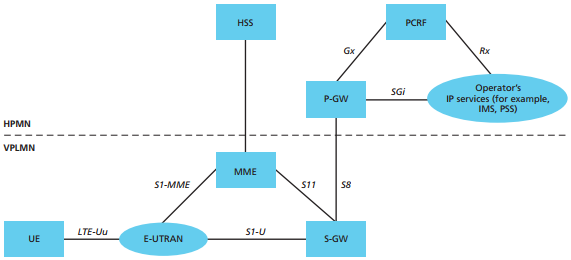
\includegraphics[width=1\linewidth]{images/Roaming}
%	\caption{Roaming Architektur \protect\cite{Ses11}}
%	\label{fig:roaming}
%\end{figure}

